%
% Article for documents at The Hague University
% of Applied Sciences, Electrical Engineering.
%
% (c)2013, J. op den Brouw <J.E.J.opdenBrouw@hhs.nl>
% v0.4
%
% Versies 0.1 - 0.3 zijn verschenen als Word-documenten
%

%% 12pt charachters, A4 paper size, one side printing, equation left aligned
%% equation indent at 0 em
\documentclass[12pt,a4paper,final,oneside,fleqn]{article}
\setlength{\mathindent}{0em}

%% PDF Version and compression...
\pdfminorversion=5
\pdfobjcompresslevel=2

%% Dutch spelling of chapter, section, etc.
\usepackage[dutch]{babel}

%% Set page layout
\usepackage[a4paper,bindingoffset=0.2in,left=1in,right=1in,top=1in,bottom=1.4in,footskip=0.6in]{geometry}

%% Allows increasing the font size of specific fonts beyond LaTeX default specifications
\usepackage{anyfontsize}

%% Use appendix
%%\usepackage{appendix}

%% Use of dashed lines in tables
\usepackage{arydshln}

%% Create text-wrapped figures and tables
\usepackage{wrapfig}

%% Include graphics files
\usepackage{graphicx}

%% Enumerate items
\usepackage{enumitem}

%% Set input encoding to ISO-8859-1 (latin1)
\usepackage[latin1]{inputenc}

%% Use the AMS Mathematical characters
\usepackage{amsmath}
\usepackage{amsfonts}
\usepackage{amssymb}

%% Use computer code listings
\usepackage{listings}

%% Define and use colors
\usepackage{color}

%% Use the Helvetica (~ Arial) font
\usepackage{helvet}

%% Use Palatino font
%%\usepackage{palatino}

%% Use the Bera Mono font encoding for listings
%%\usepackage{beramono}

%% Use the Latin Modern font... Does this change the Math font?
\usepackage{lmodern}

%% Use T1 output font encoding
\usepackage[T1]{fontenc}

%% Default monospaced font from Palatino, e.g. listings
\renewcommand{\ttdefault}{pcr}

%% Change the way chapters and sections are formatted, only sections and subsections are used
\usepackage{titlesec}
\titleformat{\section}{\fontfamily{phv}\selectfont\large\bfseries\slshape}{\thesection.}{0.5em}{}
\titleformat{\subsection}{\fontfamily{phv}\selectfont\bfseries}{\thesubsection}{0.5em}{}

%% Fancy headers and footers...
\usepackage{fancyhdr}
\pagestyle{fancy}
\lhead{}
\chead{}
\rhead{CONCEPT}
\lfoot{Coderen op de AVR}
\cfoot{}
\rfoot{\thepage}
\renewcommand{\headrulewidth}{0pt}
\renewcommand{\footrulewidth}{0.4pt}

%\renewcommand{\footnoterule}{%
%  \kern -3pt
%  \hrule width \textwidth height 1pt
%  \kern 2pt
%}

%% Indexing words...
\usepackage{makeidx}
\makeindex

%% Making captions nicer...
\usepackage[font=footnotesize,format=plain,labelfont=bf,up,textfont=it,up]{caption}

%% For using footnotes in section headers...
\usepackage[stable]{footmisc}

%% Using hyperrefs...
\usepackage{hyperref}
\hypersetup{
	colorlinks=true,
	linkcolor=blue,
    pdftitle={C coderen op de AVR},    % title
    pdfauthor={J.E.J op den Brouw},     % author
    pdfsubject={Een aantal praktische tips en voorbeelden voor goede codeertechnieken op de AVR microcontroller.},   % subject of the document
    %pdfcreator={Latex},   % creator of the document
    %pdfproducer={PDFtoLaTex}, % producer of the document
    pdfkeywords={AVR} {C coding} {tips and tricks} % list of keywords
}
\renewcommand\UrlFont{\fontfamily{phv}\selectfont\footnotesize}

%%% No package loading from here

%% Create our own maketitle macro
\makeatletter
\def\maketitle{%
  \null
  \thispagestyle{empty}%
  \vfill
  \begin{center}\leavevmode
    {\fontfamily{phv}\fontsize{30pt}{36pt}\selectfont\bfseries\scshape \@title\par}%
    \vskip 1.0cm
    {\fontfamily{phv}\fontsize{13pt}{16pt}\selectfont\bfseries\scshape \subtitle\par}%
    \vskip 8.0cm
    \begin{minipage}[c]{.50\linewidth}
       \includegraphics[width=\linewidth]{LogoHHSNederlandsGroen.png}
    \end{minipage}\hfill
    \begin{minipage}[c]{0.40\linewidth}
       {\hfill \large \@author\par}%
       \vskip 0.03cm
       {\hfill \large De Haagse Hogeschool\par}%
       \vskip 0.03cm
       {\hfill \large \@date\par}%
       \vskip 0.03cm
       {\hfill \large Versie \version\par}%
       %%\vskip 0.03cm
       %%{\hfill \Large J.E.J.opdenBrouw@hhs.nl\par}%
  \end{minipage}
  \end{center}%
  \vfill
  \null
  %%\cleardoublepage
  }
\makeatother

%% Define some colors
\definecolor{dkgreen}{rgb}{0,0.6,0}
\definecolor{gray}{rgb}{0.5,0.5,0.5}
\definecolor{mauve}{rgb}{0.58,0,0.82}
\definecolor{lightgray}{rgb}{0.95,0.95,0.95}



%% Set up listing style for C, one with and one without line numbers
\lstdefinestyle{numbers}{numbers=left, stepnumber=1, numberstyle=\small\color{gray}, numbersep=10pt}
\lstdefinestyle{nonumbers}{numbers=none}
\lstset{ %
  language=C,                           % the language of the code
  basicstyle=\footnotesize\ttfamily,    % the size of the fonts that are used for the code
  numbers=left,                         % where to put the line-numbers
  numberstyle=\small\color{gray},       % the style that is used for the line-numbers
  stepnumber=1,                         % the step between two line-numbers.
  backgroundcolor=\color{lightgray},    % choose the background color. You must add \usepackage{color}
  showspaces=false,                     % show spaces adding particular underscores
  showstringspaces=false,               % underline spaces within strings
  showtabs=false,                       % show tabs within strings adding particular underscores
  frame=lines,                          % adds framing around the code
  rulecolor=\color{black},              % if not set, the frame-color may be changed on line-breaks within not-black text (e.g. comments (green here))
  tabsize=4,                            % sets default tabsize to 4 spaces
  captionpos=b,                         % sets the caption-position to bottom
  escapeinside={(*@}{@*)},              % escape to Latex using (*@ ...  @*)
  breaklines=true,                      % sets automatic line breaking
  breakatwhitespace=false,              % sets if automatic breaks should only happen at whitespace
  aboveskip=\bigskipamount, 			%
  title=\lstname,                       % show the filename of files included with \lstinputlisting;
  morekeywords={uint8_t,uint16_t,uint32_t,ISR,asm}, % some more keywords although uint* are in fact typedefs
}

%%
%% AVRASM definition (c) 2005 Nils Michelsen
%%
\lstdefinelanguage{AVR}%
  {morekeywords={add,adc,adiw,sub,subi,sbc,sbiw,and,andi,or,ori,eor,com,neg,sbr,cbr,inc,dec,tst,
  clr,ser,mul,muls,mulsu,fmul,fmuls,fmulsu,rjmp,ijmp,eijmp,jmp,rcall,icall,eicall,call,ret,reti,
  cpse,cp,cpc,cpi,sbrc,sbrs,sbic,sbis,brbs,brbc,breq,brne,brcs,brcc,brsh,brlo,brmi,brpl,brge,brlt,
  brhs,brhc,brts,brtc,brvs,brvc,brie,brid,mov,movw,ldi,lds,ld,ldd,sts,std,lpm,elpm,spm,in,out,push,
  pop,lsl,lsr,rol,ror,asr,swap,bset,bclr,sbi,cbi,bst,bld,sec,sen,cln,sez,clz,sei,cli,ses,cls,sev,
  clv,set,clt,seh,clh,break,nop,sleep,wdr,r0,r1,r2,r3,r4,r5,r6,r7,r8,r9,r10,r11,r12,r13,r14,r15,r16,
  r17,r18,r19,r20,r21,r22,r23,r24,r25,r26,r27,r28,r29,r30,r31,tccr3a,tccr3b,tcnt3h,tcnt3l,ocr3ah,
  ocr3al,ocr3bh,ocr3bl,icr3h,icr3l,etimsk,etifr,pcmsk1,pcmsk0,clkpr,sreg,sph,spl,ucsr1c,ubrr1h,
  eimsk,gimsk,gicr,gifr,timsk,tifr,spmcr,emcucr,mcucsr,tccr0,tcnt0,ocr0,sfior,tccr1a,tccr1b,tcnt1h,
  tcnt1l,ocr1ah,ocr1al,ocr1bh,ocr1bl,tccr2,assr,icr1h,icr1l,tcnt2,ocr2,wdtcr,ubrrhi,ucsroc,ubrroh,
  eearh,eearl,eedr,eecr,porta,ddra,pina,portb,ddrb,pinb,portc,ddrc,pinc,portd,ddrd,pind,spdr,spsr,
  spcr,udr0,udr,ucsr0a,usrucsr0b,ucr,ubrr0,ubrr0l,ubrr,acsr,porte,ddre,pine,osccal,udr1,ucsr1a,
  ucsr1b,ubrr1,ubrr1l,com3a1,com3a0,com3b1,com3b0,foc3a,foc3b,wgm31,wgm30,icnc3,ices3,wgm33,wgm32,
  cs32,cs31,cs30,icf3,ocf3a,ocf3b,tov3,pcint15,pcint14,pcint13,pcint12,pcint11,pcint10,pcint9,
  pcint8,pcint7,pcint6,pcint5,pcint4,pcint3,pcint2,pcint1,pcint0,CLKPCE,CLKPS3,CLKPS2,CLKPS1,CLKPS0,
  INT1,INT0,INT2,PCIE1,PCIE0,IVSEL,IVCE,INTF1,INTF0,INTF2,PCIF1,PCIF0,TOIE1,OCIE1A,OCIE1B,OCIE2,
  TICIE1,TOIE2,TOIE0,OCIE0,TOV1,OCF1A,OCF1B,OCF2,ICF1,TOV2,TOV0,OCF0,SPMIE,RWWSB,ASB,RWWSRE,ASRE,
  BLBSET,PGWRT,PGERS,SPMEN,SM0,SRL2,SRL1,SRL0,SRW01,SRW00,SRW11,ISC2,SRE,SRW,SRW10,SE,SM,SM1,ISC11,
  ISC10,ISC01,ISC00,JTD,SM2,JTRF,WDRF,BORF,EXTRF,PORF,FOC0,WGM00,PWM0,COM01,COM00,WGM01,CTC0,CS02,
  CS01,CS00,TSM,XMBK,XMM2,XMM1,XMM0,PUD,PSR2,PSR10,PSR1,PSR0,COM1A1,COM1A0,COM1B1,COM1B0,FOC1A,
  FOC1B,PWM11,WGM11,PWM10,WGM10,ICNC1,ICES1,CTC11,WGM13,CTC10,WGM12,CTC1,CS12,CS11,CS10,FOC2,WGM20,
  PWM2,COM21,COM20,WGM21,CTC2,CS22,CS21,CS20,AS2,TCN2UB,OCR2UB,TCR2UB,WDTOE,WDCE,WDE,WDP2,WDP1,
  WDP0,EERIE,EEMWE,EEWE,EERE,PORTA7,PORTA6,PORTA5,PORTA4,PORTA3,PORTA2,PORTA1,PORTA0,DDA7,DDA6,
  DDA5,DDA4,DDA3,DDA2,DDA1,DDA0,PINA7,PINA6,PINA5,PINA4,PINA3,PINA2,PINA1,PINA0,PORTB7,PORTB6,
  PORTB5,PORTB4,PORTB3,PORTB2,PORTB1,PORTB0,DDB7,DDB6,DDB5,DDB4,DDB3,DDB2,DDB1,DDB0,PINB7,PINB6,
  PINB5,PINB4,PINB3,PINB2,PINB1,PINB0,PORTC7,PORTC6,PORTC5,PORTC4,PORTC3,PORTC2,PORTC1,PORTC0,
  DDC7,DDC6,DDC5,DDC4,DDC3,DDC2,DDC1,DDC0,PINC7,PINC6,PINC5,PINC4,PINC3,PINC2,PINC1,PINC0,PORTD7,
  PORTD6,PORTD5,PORTD4,PORTD3,PORTD2,PORTD1,PORTD0,DDD7,DDD6,DDD5,DDD4,DDD3,DDD2,DDD1,DDD0,PIND7,
  PIND6,PIND5,PIND4,PIND3,PIND2,PIND1,PIND0,PORTE2,PORTE1,PORTE0,DDE2,DDE1,DDE0,PINE2,PINE1,PINE0,
  RXC,TXC,UDRE,FE,OR,U2X,RXC0,TXC0,UDRE0,FE0,OR0,DOR0,PE0,U2X0,MPCM0,RXC1,TXC1,UDRE1,FE1,OR1,DOR1,
  PE1,U2X1,MPCM1,SPIE,SPE,DORD,MSTR,CPOL,CPHA,SPR1,SPR0,SPIF,WCOL,SPI2X,RXCIE,TXCIE,UDRIE,RXEN,
  TXEN,CHR9,UCSZ2,RXB8,TXB8,RXCIE0,TXCIE0,UDRIE0,RXEN0,TXEN0,CHR90,UCSZ02,RXB80,TXB80,RXCIE1,TXCIE1,
  UDRIE1,RXEN1,TXEN1,CHR91,UCSZ12,RXB81,TXB81,URSEL0,UMSEL0,UPM01,UPM00,USBS0,UCSZ01,UCSZ00,UCPOL0,
  URSEL1,UMSEL1,UPM11,UPM10,USBS1,UCSZ11,UCSZ10,UCPOL1,ACD,AINBG,ACBG,ACO,ACI,ACIE,ACIC,ACIS1,
  ACIS0,BLB12,BLB11,BLB02,BLB01,XL,XH,YL,YH,ZL,ZH,RAMEND,EEPROMEND,FLASHEND,SMALLBOOTSTART,
  SECONDBOOTSTART,THIRDBOOTSTART,LARGEBOOTSTART,BOOTSTART,PAGESIZE,INT0addr,INT1addr,INT2addr,
  PCINT0addr,PCINT1addr,TIMER3CAPTaddr,TIMER3COMPAaddr,TIMER3COMPBaddr,TIMER3OVFaddr,TIMER2COMPaddr,
  TIMER2OVFaddr,TIMER1CAPTaddr,TIMER1COMPAaddr,TIMER1COMPBaddr,TIMER1OVFaddr,TIMER0COMPaddr,
  TIMER0OVFaddr,SPISTCaddr,USART0RXCaddr,USART1RXCaddr,USART0UDREaddr,USART1UDREaddr,USART0TXCaddr,
  USART1TXCaddr,EE_RDYaddr,ANA_CMPaddr,SPM_RDYadd,org,def,equ,db,include,dseg,cseg,eseg,mcucr,
  ubrr0h,ucsr0c,ucsr0b},
   sensitive=f,
   morecomment=[l];,%
   morestring=[d]{"}%
  }[keywords,comments,strings]%


%% Ahhhh... At last, the beginning of the document...
\begin{document}
\author{Jesse op den Brouw}
\title{C coderen op de AVR}
\newcommand{\subtitle}{Een aantal praktische tips en voorbeelden voor goede codeertechnieken op de AVR microcontroller.}
\date{\today}
\newcommand{\version}{0.4}

%% Make title page
\maketitle

%% Make table of contents
\newpage
\tableofcontents
\vfill
\noindent
\begin{center}
Vragen en commentaar over dit document kunnen worden gestuurd naar
\href{mailto:J.E.J.opdenBrouw@hhs.nl}{J.E.J.opdenBrouw@hhs.nl} of in
geschreven vorm worden aangeboden in kamer D1.047.
\end{center}

%% Make a list of listings
\newpage
\lstlistoflistings

%% The first section
%% We begin at section 0.
\setcounter{section}{-1}
\newpage
\thispagestyle{fancy}
\section{Hoe codeer je het beste op een AVR?}
De vraag is heel simpel gesteld, maar het antwoord is natuurlijk niet
zomaar te geven.
De titel suggereert dat dit document het ultieme antwoord is op
alle vragen die gesteld kunnen worden over het coderen op de AVR-serie.
Dat is natuurlijk niet waar. 

Dit document behandelt een aantal aspecten van het coderen van software.
Het gaat hier om hoe code wordt gepresenteerd, hoe je bepaalde valkuilen
kunt omzeilen maar niet zozeer om een daadwerkelijke implementatie van een
algoritme. Daarnaast blijkt dat de AVR-controller een intrigerende, maar
vooral lastige processor is voor beginnende programmeurs. Veel problemen
komen voort uit het gebruik van de specifieke hardware, zoals timers en
seri\"{e}le poorten. Ook hier zijn tips over opgenomen.

Een aantal van deze tips komt voort uit de jarenlange colleges en practica
die gegeven worden aan studenten van de opleiding Elektrotechniek aan De
Haagse Hogeschool te Delft. Tijdens de lessen wordt gebruik gemaakt van
AVR-Studio versie 4 (versie 6 is in voorbereiding), de WinAVR C-compiler,
de STK500, de JTAGICE-mkII en een ATmega32. Daarnaast is een eigen
opsteekprint gemaakt met een LCD en potmeter voor gebruik van de ADC. Er is
een website beschikbaar waarop het hele curriculum, inclusief PowerPoint-
presentaties en practicumopdrachten is ondergebracht. Surf maar naar
\url{http://bd.eduweb.hhs.nl/micprg/}.

C is een geweldige taal, je kan er ontzettend veel mee doen als je een
microcontrollerbordje programmeert. Maar C heeft \'{e}\'{e}n nadeel: het
legt de programmeer geen regels op voor het netjes vormgeven van de code.
Je kan het hele programma, met uitzondering van de preprocessorregels, als
\'{e}\'{e}n lange regel aan de compiler aanbieden: niet leesbaar, wel
compileerbaar. Wil je meer weten van totaal niet leesbare code, ga dan naar
\url{http://www0.us.ioccc.org/main.html}.

\newpage
\section{Denk eerst na voor je code gaat schrijven.}

Da's natuurlijk een mooie binnenkomer, maar zeker niet onbelangrijk. Eerst
nadenken over je probleem en vervolgens je code schrijven werkt veel beter
dan ``gewoon beginnen en zien tot hoever we komen''. Beschrijf wat de code
moet doen en ontwerp alvast een soort framewerk waarbinnen alles moet passen.

\begin{lstlisting}[style=numbers,caption=Voorbeeld van een framework]
uint16_t haal_ADC_waarde(void) {
}

void start_ventilator(void) {
}

uint8_t is_klep_gesloten(void) {
}

enum (begin_st, klep_dicht_st, tapkraan_aan_st) ;

int main(void) {

	while (1) {
		switch (toestand) {
			case begin_st:         break;
			case klep_dicht_st:    break;
			case tapkraan_aan_st:  break;
		}
	}
	return 0;
}
\end{lstlisting}


\section{Schrijf duidelijke code.}

Da's natuurlijk nog een leuke binnenkomer, maar ook zeker niet minder waar.
C heeft een aantal zeer mooie schrijfwijzen, zoals de ++-operator en alle
toekenningsvarianten. Constructies als:

\begin{lstlisting}[style=nonumbers,belowcaptionskip=-12pt]
for (int i=0,j=10; ++i<j-2; j++) {	 ... }

list[i++]&=(*(pint++)|(1<<5));
\end{lstlisting}

\noindent
zijn niet te volgen, het is beter om ze uit te schrijven. Dit levert weliswaar
meer broncode op, maar de compilers zijn tegenwoordig zo goed, dat de resulterende
assemblercode minimaal is. Anderzijds is

\begin{lstlisting}[style=nonumbers,belowcaptionskip=-12pt]
TIMSK|=0x04;
\end{lstlisting}

\noindent
weer minder goed te lezen (en zeker minder portable) dan

\begin{lstlisting}[style=nonumbers,belowcaptionskip=-12pt]
TIMSK|=(1<<TOIE1);
\end{lstlisting}

\section{Laat duidelijk zien op welke niveau de code thuis hoort.}
Met niveau wordt het inspringen bedoeld (engels: indentation), gebruikmakend van
de TAB-toets. De meeste editors hebben een tab-afstand van 4 of 8 spaties. Een
functie zoals \texttt{main} ligt op niveau 0; dit ligt aan het begin van de regel.
De code in een functie begint dus altijd op niveau 1. Statements zoals \texttt{if},
\texttt{while} en \texttt{for} leveren een niveau extra op, zoals te zien is in het
voorbeeld. De verschillende niveau's zijn goed te volgen.

\begin{lstlisting}[style=numbers,caption=Voorbeeld van code met inspringen]
int main() {                                // niveau 0

	...
	if (flag==1) {                          // niveau 1
		while (PORTB&0x01) {                // niveau 2
			for (i=0; i<8; i++) {           // niveau 3
				PORTA = 0x01;               // niveau 4
				wait();                     // niveau 4
				PORTA = 0x00;               // niveau 4
				wait();                     // niveau 4
			}                               // niveau 3
		}                                   // niveau 2
		PORTA = 0x80;                       // niveau 2
	}                                       // niveau 1

	return 0;                               // niveau 1
}                                           // niveau 0

void wait() {                               // niveau 0

	int i;                                  // niveau 1

	for (i=0; i<30000; i++) {               // niveau 1
		nop();                              // niveau 2
	}                                       // niveau 1
}                                           // niveau 0
\end{lstlisting}

\section{Gebruik \#define voor constanten en parameters die door de gebruiker zijn aan te passen.}
Niets is zo heerlijk als door je hele programma het getal '10' te moeten vervangen,
omdat je nu besloten hebt dat je array 20 tekens mag bevatten. Een simpele

\begin{lstlisting}[style=nonumbers,belowcaptionskip=-12pt]
#define BUF_LEN 10
\end{lstlisting}

\noindent
bespaart een hoop ellende. Veel mooier is om gebruikersparameters (nou ja, voor degene
die de code compileert en gebruikt) in een aparte header-file op te nemen die te laten includen.

\begin{lstlisting}[style=nonumbers,caption=Voorbeeld header file met User Preferences]
#define F_CPU 3686400UL
#define PRESCALER 1024UL
#define FREQ 4UL
\end{lstlisting}

\noindent
In een andere header-file (of C-file) wordt deze file dan ingelezen.

\begin{lstlisting}[style=nonumbers,caption=Gebruik van header file]
#include "user_pref.h"
#ifndef F_CPU
#define F_CPU 3686400UL
#warning F_CPU set to 3.6864 MHz
#endif

#define COUNT ((F_CPU)/((PRESCALER)*(FREQ)))
#define LOAD (65536-(COUNT))

ISR(...) {
	TCNT1 = LOAD;
	...
}
\end{lstlisting}

\section{Gebruik enum voor variabelen die niet door de gebruiker zijn 
aan te passen en maar enkele waarden kunnen aannemen.}
Typisch voorbeeld hiervan zijn de toestanden van een toestandsmachine.
Je kan zelf een nieuw type aanmaken met \texttt{typedef}.

\begin{lstlisting}[style=numbers,caption=Voorbeeld van een toestandsmachine]
/* The states of the state machine */
typedef enum {Idle, Wait1, Fetch, Temp, Load, Store} state_t;

/* Startup state */
state_t s=Idle;

int main(void) {

	/* Do forever */
	while (1) {
		switch (s) {
			case Idle:
			case Wait1:
			case Fetch:
			default:
				state = Idle;
				break;
		}
	}
}
\end{lstlisting}

\section{Regels voor naamgeving.}
Ieder bedrijf, projectgroep, programmeur heeft ongetwijfeld zijn eigen stijl
met betrekking tot het geven van namen, maar neem een aantal regels in acht:

\begin{enumerate}[align=left,itemsep=0cm,leftmargin=*,label=\Roman*.]
\item Namen met leidende underscores zijn gereserveerd voor systeemdoeleinden
en moeten niet gebruikt worden voor variabele-namen.
\item \texttt{\#define} constanten moeten allemaal met HOOFDLETTERS geschreven
worden.
\item Enum constanten moeten allemaal met HOOFDLETTERS geschreven worden, of
beginnen met een Hoofdletter.
\item Functie-, \texttt{typedef}-, en variabelennamen, als ook \texttt{struct},
\texttt{union}, en \texttt{enum} tag-namen moeten met kleine letters geschreven worden.
\item Typedeffed namen eindigen met \texttt{\_t}.
\item Lange namen kunnen opgedeeld worden met behulp van underscores of het
gebruik van hoofdletters: \texttt{counter\_for\_indexing} of \texttt{counterForIndexing}.
Dat laatste wordt de \textit{camelCase} genoemd, waarbij de eerste
letter met een kleine letter geschreven worden.
\end{enumerate}


\section{Gebruik duidelijke variabelennamen.}
De beroemde \'{e}\'{e}nletterige variabelennamen zijn natuurlijk uit den boze.
Als lusteller misschien nog wel, maar voor de rest niet. De C-compiler kan
variabelennamen tot 31 tekens verwerken\cite{isocdraft2005}, maar dat kost jou wel
veel typewerk. Nog wat regels.

\begin{enumerate}[align=left,itemsep=0cm,leftmargin=*,label=\Roman*.]
\item Vermijd namen die slechts in hoofdletters en kleine letters verschillen,
  zoals \texttt{foo} en \texttt{Foo}.
\item Vermijd namen die in bibliotheken voorkomen zoals \texttt{read} en \texttt{write}.
\end{enumerate}

\noindent
Hieronder een tweetal links: \\
\url{http://www.ibm.com/developerworks/linux/library/l-clear-code/} \\
\url{http://www.doc.ic.ac.uk/lab/cplus/cstyle.html}


\section{Voeg commentaar toe aan de code.}
-- the source is the documentation -- is een veel gehoorde uitspraak. En dat is jammer,
want goede documentatie zorgt veel het sneller begrijpen van de code. Het is niet zinvol
om achter elke regel die ene statement uit te leggen:

\begin{lstlisting}[style=nonumbers,belowcaptionskip=-12pt]
i++;		/* Verhoog i */
\end{lstlisting}

\noindent
snappen de meesten van ons ook wel. Beter is het om een klein stukje code dat een
afgebakende functie heeft, te begeleiden met een paar regels commentaar. Zie voorbeeld.

\begin{lstlisting}[style=numbers,caption=Code met commentaar]
/*
 * This routine will bit-bang the least significant
 * bit of Port A, on which the device's clock line is
 * connected, for 8 times until the device will
 * respond with a reset (lsb on Port B). Then, the
 * restart command, a 1 on the msb of Port A, will be
 * asserted. After this the device will be in a
 * known (reset) state.
*/
while (PORTB&0x01) {
		for (i=0; i<8; i++) {
			PORTA = 0x01;
			wait();
			PORTA = 0x00;
			wait();
		}
}
PORTA = 0x80;
\end{lstlisting}

\section{Doe foutafhandeling.}
Ook jij maakt fouten. Dus zul je ze moeten afhandelen. Maar nog erger zijn je
gebruikers. Niet gehinderd door enige kennis van zaken zullen deze personen
alles proberen om je programma om zeep te helpen. Denk hier aan: invoer die niet
voldoet aan gestelde eisen, zoals alleen cijfers invullen of een getal groter dan
0 en kleiner dan 1000, states waar je toestandmachine nooit in mocht komen, namen
van files die niet bestaan. Het gebruik van de \texttt{if}-statement met goede
afhandelingscode is hier natuurlijk voor bedoeld.

\section{Vermijd gebruik van floating point.}
De AVR-controller heeft geen hardware voor floating point-berekeningen aan boord.
Dat betekent dat zelfs een simpele vermenigvuldiging of deling in software moet
worden ge\"{e}muleerd. En dat kost veel ruimte in ROM en veel executietijd. Onderstaande
code werd gedraaid op een ATmega16 met GNU-C compiler versie 4.1. De floating point-berekeningen
duren meer dan twee keer zo lang als de integer-berekeningen. Het gebruik van de
optimalisatievlag \texttt{-O2} helpt weinig (zeg maar gewoon: niets) want de routines
voor vermenigvuldigen en delen zijn al geoptimaliseerd door de programmeurs.
Je kan veel eenvoudige floating point-delingen makkelijk omzetten naar integer-delingen
(let wel op het bereik van int's en long's) (let ook op de berekenvolgorde!):

\begin{equation}
\nonumber
fo = \frac{ftime}{fdiv}=\frac{ftime}{3,686} \quad \Rightarrow \quad
lo = \frac{ltime \cdot lmul}{ldiv} = \frac{ltime \cdot 1000}{3686} \qquad
\left(\frac{1}{3,686} \leftrightarrow \frac{1000}{3686}\right)
\end{equation}

\begin{lstlisting}[style=numbers,caption=Code met integer en floating point-berekeningen]
/* compile with -O0 and -O2 successively */

volatile float fx=13.0;
volatile float fy=23.535;
volatile float fz;

volatile long  lx=13UL;
volatile long  ly=23535;
volatile long  lz;

volatile long   ftime = 3456;
volatile float  fdiv = 3.686;
volatile float  fo;

volatile long   ltime = 3456;
volatile long   lmul = 1000;
volatile long   ldiv = 3686;
volatile long   lo;

int main() {

	fz = fy/fx;

	lz = ly/lx;

	fo = ftime/fdiv;

	lo = (ltime*lmul)/ldiv;    /* Mind parentheses!!! */

	return 0;
}
\end{lstlisting}

\noindent
Let ook op het gebruik van \texttt{\#define}-constanten. Constucties als

\begin{lstlisting}[style=nonumbers,belowcaptionskip=-12pt]
#define R_OPT (14750.0)
\end{lstlisting}

\noindent
levert extreem veel code op omdat er t\'{o}ch FP-routines worden gebruikt.


\section{Let op het gebruik van gemeenschappelijke variabelen.}
\label{sec:gemvar}
In de wereld van Operating Systems is er een probleem met variabelen
die gemeenschappelijk gebruikt worden door twee of meer processen.
Hier kan het updaten van variabelen door deze processen soms tot foutieve
uitkomsten leiden. Maar de AVR is een processor waarop standaard geen OS
draait. Dat betekent dat je alles in de hand hebt. Dus waar maken we ons
zorgen om? Welnu, als je gebruik maakt van Interrupt Service Routines (ISRs),
dan heb je eigenlijk een processor (de AVR) met daarop twee processen:
de eigen \texttt{main()} en de ISR. De ISR wordt namelijk door een hardware-gebeurtenis
gestart asynchroon met het hoofdprogramma. Terwijl het hoofdprogramma een
variabele aan het aanpassen is, wordt de ISR aangeroepen die die variabele
\'{o}\'{o}k aanpast. Dat is vragen om ellende. Hier geldt ook voor: het is niet de
vraag \'{o}f het gebeurt, maar wanneer! Zie onderstaande code.

\begin{lstlisting}[style=numbers,caption=Afschermen van gemeenschappelijke variabelen]
ISR(TIMER1_COMPA_vect) {

	/* ... more code ... */
	
/* toggle LED, this is atomically because the */
/* ISR cannot be interrupted */
	PORTB=PORTB^(1<<LED);
}

int main() {

	if (...) {
		/* Bad!                                   */
		/* Assember code for next statement is:   */
		/*    in   r24,PORTB                      */
		/*    ori  r24,0xf0                       */
		/*    out  PORTB,r24                      */
		/* Things go wrong when interrupt occurs  */
		/* directly after the in-instruction      */
		/* because R24 now holds a COPY of PORTB! */
		PORTB=PORTB|0xf0;
	}

	if (...) {
		/* Good!                                      */
		/* Make PORTB operation atomically by cli/sei */
		cli();
		PORTB=PORTB|0xf0;
		sei();
	}		

	return 0;
}
\end{lstlisting}

\section{Maak gebruik van functies voor het aan- en uitschakelen van de hardwaresturing.}
Code wordt beter leesbaar als er een aanroep wordt gedaan naar \texttt{activeer\_pomp()}
dan \texttt{PORTB|=0x40}. De inhoud van \texttt{activeer\_pomp()} is dan zeer klein, maar
dat moet niet uit maken. Als je optimalisatie \texttt{-O3} gebruikt heb je grote kans dat
de compiler de functies helemaal niet aanmaakt maar de body van de functies plaatst op
de plek van de aanroep (inline). Bij herhaald gebruik kost dit iets meer ruimte, maar
levert wel een tijdbesparing omdat het aanroepen en terugkeren van de functie wordt vermeden.

\begin{lstlisting}[style=numbers,caption=Voorbeeld gebruik functies voor hardwaresturing]
#define POMP_BIT 6

void PompAan() {
	PORTB|=(1<<POMP_BIT);
}

void PompUit() {
	PORTB&=~(1<<POMP_BIT);
}

int main() {

	if (s==Load) {
		PompAan();
	} else {
		PompUit();
	}

	return 0;
}
\end{lstlisting}


\section{Plaatsing van accolades.}
Dit is altijd het gevecht tussen twee kampen: zij die de accolades achter
\texttt{if}, \texttt{for}, \texttt{while} en \texttt{switch} zetten en zij die het
eronder zetten. Beide zijn goed, maar houd je wel aan \'{e}\'{e}n vorm en ga ze
niet door elkaar gebruiken. Nog een tip: ook \texttt{if}, \texttt{for},
\texttt{while}-statements met slechts \'{e}\'{e}n regel code moet je tussen
accolades zetten. Da's handig voor later als je beslist om er nog wat regels
code bij te plaatsen, want d\'{a}n vergeet je ze natuurlijk.

\begin{lstlisting}[style=numbers,caption=Plaatsing van accolades]
/* Use with functions! */
void test()
{
	/* Variant 1 */
	if (a==b) {
		c=d;
		d=d+1;
	} else {
		c=c+1;
		d=c;
		k=k2;
	}

	/* Variant 2 with only one statement with {} */
	if (c==d)
	{
		a=b;
	}
	else
	{
		a=f;
	}
}

int main(void) {

	test();
	return 0;
}
\end{lstlisting}


\section{Interruptroutines moeten zo snel mogelijk uitgevoerd worden.}
\label{sec:intsnel}
Een interrupt is een onderbreking van het lopende programma. De hardware
van de AVR signaleert dat er iets gebeurd is zoals een timer die over de
kop gaat (overflow) of de ADC die klaar is met een nieuwe conversie. Als
een Interrupt Service Routine (ISR) wordt uitgevoerd ligt het lopende
programma stil. Als hier besturing in is geprogrammeerd, bijvoorbeeld van
een robot, is het programma dus niet in staat de robot te sturen. ISR's
moeten daarom zo snel mogelijk worden uitgevoerd. Dit betekent dat je bv.
geen floating-point-berekeningen moet uitvoeren of de LCD-display moet
aansturen, maar ook geen lus die blijft wachten tot een variabele is
veranderd. Korte lusjes, bijvoorbeeld om een array te initialiseren is
geen probleem. Probeer de executie-tijd van een ISR (ruim) onder de 100
$\mu$s te houden. Dit kan je prima testen met de simulator.

\begin{lstlisting}[style=numbers,caption=ISR's moeten kort duren]
double x, y, angle;
uint16_t adc_val[10];

ISR(TIMER1_COMPA_vect) {

	/* BAD! Waits for bit change */
	while (PORTA&=0x80);

	/* OK */
	PORTB=PORTB^(1<<LED);

	/* BAD ! Uses LCD. Takes a long time */
	lcd_puts("In T/C1 ISR.\n");

	/* BAD ! Takes a long time, are double operations */
	x = cos(angle); y = sin(angle);

	/* OK, it is a loop, but doesn't take a long time */
	for (i=0; i<10; i++) { adc_val[i]=0; }
}

int main() {

	lcd_init();
	...
	...
	
	return 0;
}
\end{lstlisting}

%% Verwijderd. Hoeveelheid code is in principe niet van belang, uitvoersnelheid wel.
%%\section{Interruptroutines moeten zo min mogelijk code bevatten.\footnote{dispuut met Harry}}
%%Eigenlijk klinkt dit logisch als je naar de vorige regel kijkt. Minder code betekent
%%meestal snelle uitvoering. In veel gevallen kan je de ISR gebruiken om een gebeurtenis
%%te signaleren met behulp van een simpele (\'{e}\'{e}n byte) variabele, ook wel flag genoemd.
%%Denk hierbij aan alarmmeldingen! Het hoofdprogramma test dan deze flag en doet hierna
%%de bedoelde actie. Zie ook \ref{sec:atomair}.

\section{Test gebeurtenissen als atomaire actie.}
\label{sec:atomair}
Merk op dat de test en op nul zetten van de flag (gebeurtenis is gezien) wordt afgeschermd
met een \texttt{cli}/\texttt{sei}-paar. Dit is een equivalent van een test-and-set-instructie.
Hierdoor voorkom je dat de ISR de flag weer op \'{e}\'{e}nn zet v\'{o}\'{o}r het uitvoeren van
de ''zet op nul''-instructie met als gevolg dat een gebeurtenis niet wordt gezien. Zie voorbeeld.
Zie ook \ref{sec:gemvar}.

\begin{lstlisting}[style=numbers,caption=Atomaire acties]
#include <avr/interrupt.h>
#include <stdint.h>

/* Note: only one-byte variable! */
volatile uint8_t adc_ready=0;
volatile uint16_t adc_val=0;

ISR(ADC_vect) {

	/* Flag ADC has a new value */
	adc_ready = 1;
    adc_val = ADC;

	/* Start new conversion, use with simulator */
	/* ADCSRA |= (1<<ADSC); */
}

int main() {

	uint16_t temp=0;

	/* Set up ADC */
	ADMUX = 0b00000000;
	ADCSRA = (1<<ADEN)|(1<<ADSC)|(1<<ADATE)|(1<<ADIF)|
	            (1<<ADIE)|(1<<ADPS2)|(1<<ADPS1)|(1<<ADPS0);

	/* Do forever */
	while (1) {

		/* Block interrupts. Interrupts must be blocked,  */
		/* because there is a possibility that the ISR is */
		/* invoked just after the if-statement and before */
		/* the assignment, in which case we would miss an */
		/* event from the ISR.....                        */
		cli();
		/* Is ADC ready? */
		if (adc_ready == 1) {
			/* Reset flag for next time */
			adc_ready = 0;
			/* Free interrupts */
			sei();
			/* More stuff, probably with the ADC */
			/* Calculate temp from an AD592 temp-sensor */
			temp = ((adc_val-559)*100)/204;
		} else {
			/* Free interrupts (don't forget here!) */
			sei();
		}
	}

	return 0;
}
\end{lstlisting}

\section{Volatile.}
Een veel gebruikte oplossing voor het signaleren van een interrupt is
de flag-variabele: een variabele wordt op \'{e}\'{e}n gezet in een ISR
en getest en op nul gezet in \texttt{main()}. Dit is een prima methode. \\
De huidige compilers zijn echter erg slim. Een ISR wordt nooit aangeroepen
door een software-instructie maar door een hardwaregebeurtenis. Een compiler
kan dan beslissen om de flag helemaal weg te laten, immers de ISR wordt toch
nooit aangeroepen en dus nooit uitgevoerd. Maar dan kan de compiler ook
beslissen om de test-en-op-nul-zet actie in \texttt{main()} er uit te laten.
De flag variabele wordt toch nooit \'{e}\'{e}n. \\
Om dit te voorkomen moet bij de declaratie van de flag het keyword
\texttt{volatile} worden opgegeven wat zoveel wil zeggen als: compiler, blijf
met je vingers van de variabele af want er gebeurt iets onder de motorkap
waar jij geen weet van hebt. \\
Het nadeel is nu dat de compiler bij elke actie
met die flag de waarde uit het RAM-geheugen moet ophalen waardoor langere
executietijden ontstaan. Gebruik \texttt{volatile} daarom ook alleen als het
nodig is. Als je in een ISR een \texttt{volatile}-variabele vaak nodig hebt,
kan het soms slim zijn om die \texttt{volatile}-variabele te kopi\"{e}ren
naar een gewone, non-\texttt{volatile}-variabele en dan verder de
gewone variabele gebruiken. Optimalisatie zorgt er voor dat de gewone
variabele \'{e}\'{e}n keer geladen wordt en vervolgens in een register
vastgehouden wordt tijdens de uitvoer van de ISR. Je codeert nu meer
C-code, met als resultaat dat de gegenereerde machinecode kleiner is!
Als je de optimalisatie van de compiler uitzet, heb je grote kans dat
\texttt{volatile} niet nodig is omdat de compiler dan in een ''domme'' modus
staat, maar er is geen garantie. \\
Zie als voorbeeld de code bij \ref{sec:atomair}.


\section{Gebruik zo min mogelijk bronnen (resources).}
%%\footnote{dispuut met Harry}}
Naast dat je natuurlijk een zo'n klein mogelijk programma moet coderen en zo min
mogelijk RAM-geheugen moet gebruiken, is het verstandig om \'{o}\'{o}k te
besparen op hardwarebronnen. Een veel voorkomend gebruik is om twee timers
te nemen als twee tijden (tijdspannen) moeten worden bijgehouden. Een voorbeeld
hiervan is een led elke seconde te laten knipperen en de ADC elke tien seconden
een conversie te laten doen. Veel van deze problemen kunnen prima met
\'{e}\'{e}n timer worden opgelost. De truuk is om met \'{e}\'{e}n
hardware-timer meerdere software-timers te maken. \\

Op de volgende pagina's is een typische toepassing geprogrammeerd. Timer/Counter
0 (T/C0) wordt gebruikt als tijdmeter. Elke 100\textsuperscript{ste} van een
seconde wordt de Interrupt Service Routine (ISR) van T/C0 aangeroepen (de Compare
Match ISR om precies te zijn). E\'{e}n teller houdt bij hoeveel
100\textsuperscript{sten} van een seconde voorbij zijn. Als dat er precies 100
zijn is 1 seconde tijd verstreken. Op dat moment worden twee andere tijden, te
weten een tijdmeter van 3 seconden en \'{e}\'{e}n van 7 seconden aangepast. Is
ook die tijd verstreken (het zijn dus twee onafhankelijke tijdmeters), dan wordt
een actie ondernomen. In het voorbeeld worden twee leds getoggeld. Merk op dat
T/C0 slechts een 8 bit telregister heeft. Het is bijvoorbeeld niet mogelijk om
10\textsuperscript{den} van seconden in \'{e}\'{e}n keer te tellen bij gegeven
frequentie.

\begin{lstlisting}[style=numbers,caption=Meerdere software timers d.m.v. een hardware timer]
//Include the two needed header files
#include <avr/io.h>
#include <avr/interrupt.h>

// There are two time, at 3 and 7 seconds
#define TIME1 3
#define TIME2 7

// Check for CPU frequency set, or bail out
#ifndef F_CPU
#error Please set CPU frequency in the project options.
#endif

// Timer frequency is 100 Hz, prescaler and prescaler bits
#define FREQ 100UL
#define PRESCALER 1024
#define PRESCALER_BITS ((1<<CS02)|(1<<CS00))

// Nice trick if you need a debug point ;-)
#define nop() asm volatile ("nop" ::)

// The three time keepers.
uint8_t time1_tick = 0;
uint8_t time2_tick = 0;
uint8_t hundredths = 0;

// The Interrupt Service Routine for T/C0 compare match
ISR(TIMER0_COMP_vect) {

	// Increment hundredths of seconds
	hundredths++;
	if (hundredths == FREQ) {
		// We have one second now
		hundredths = 0;
		time1_tick++;
		if (time1_tick == TIME1) {
			// We have Time 1 now...
			time1_tick = 0;
			PORTB^=(1<<PB7);
		}
		time2_tick++;
		if (time2_tick == TIME2) {
			// We have Time 2 now...
			time2_tick = 0;
			PORTB^=(1<<PB6);
		}
	}
}

// Main, as in every C program
int main() {

	// Initialize T/C0 to Compare Match mode with ISR
	TIMSK = (1<<OCIE0);
	TIFR  = (1<<OCF0);
	TCCR0 = (1<<WGM01) | PRESCALER_BITS;
	OCR0  = ((F_CPU/PRESCALER)/FREQ)-1;

	// Port B is leds output
	DDRB  = 0xff;
	PORTB = 0xff; // For STK500

	// Free interrupts
	sei();

	while (1) {
		// You can set a breakpoint here.....
		nop();
	}

	// Yeah, yeah, never reached
	return 0;
}
\end{lstlisting}

%%\section{Schrijf robuuste code}

\section{Gebruik Flash ROM geheugen voor lange strings}
Als je veel tekst hebt af te drukken, bijvoorbeeld via de RS232-interface
of via de lcd, dan is het niet handig om de tekst ''gewoon'' op te slaan als
een string. De tekens van de strings moeten met het programma mee in de
AVR geflashd worden, dus die tekens staan in de Flash-ROM. Als het programma
start worden de tekens naar RAM gekopi\"{e}erd, nog voordat \texttt{main()}
wordt aangeroepen. Aangezien de ATmega's niet zo heel veel RAM aan boord
hebben, is het beter om de strings in ROM te laten staan en de
tekens op te halen via de \texttt{pgm\_read\_*}-functies te benaderen.
Documentatie is te vinden in \cite{avrlibc2012}

\begin{lstlisting}[style=numbers,caption=Gebruik van PROGMEM strings]
/*********************************************
* Chip type           : ATmega32A
* Clock frequency     : 3.6864 MHz
*********************************************/
#include <avr/io.h>
#include <avr/interrupt.h>
#include <inttypes.h>
#include <avr/io.h>
#include <avr/pgmspace.h>

/* Note: define F_CPU in Configuration Options */
#define USART_BAUD_RATE 9600
#define USART_BAUD_CALC(USART_BAUD_RATE,F_CPU) \
		((F_CPU)/((USART_BAUD_RATE)*16l)-1)

/* Define strings in Program Memory (Flash) using PROGMEM */
char welcome1[] PROGMEM = "Welcome to AVR ATmega32A.......\r\n";
char welcome2[] PROGMEM = "Type some text to see the copy.\r\n";

/* Initialize the USART */
void usart_init(void) {
	/* Set baud rate */
	UBRRH = (uint8_t)(USART_BAUD_CALC(USART_BAUD_RATE,F_CPU)>>8);
	UBRRL = (uint8_t)USART_BAUD_CALC(USART_BAUD_RATE,F_CPU);

	/* Enable the transmitter and receiver, no interrupts */
	UCSRB = (1<<RXEN)|(1 << TXEN);

	/* Asynchronous 8N1 */
	UCSRC = (1 << URSEL) | (3 << UCSZ0);
}

/* Wait for a character reception */
char usart_getc(void) {
	/* Wait until receiver has data */
	while(!(UCSRA & (1 << RXC)));
	/* Return character */
	return UDR;    
}

/* Transmit a character */
void usart_putc(char c) {
	/* Wait until transmitter is ready to send data */
	while(!(UCSRA & (1 << UDRE)));
	/* Send character */
	UDR = c;    
}

/* Transmit a PROGMEM string */
void usart_puts_P(char *s) {

	uint8_t ch;
	while ( (ch = pgm_read_byte(s)) != '\0') {
		usart_putc(ch);
		s++;
	}
}

int main(void) {

	char c;

	usart_init(); /* init USART */
	
	/* Send greeting text */
	usart_puts_P(welcome1);
	usart_puts_P(welcome2);

	/* Forever copy input to output */
	while (1) {
		/* Read character */
		c = usart_getc();
		/* If the character is a CR, send CR & LF */
		if (c == '\r')
			usart_puts_P(PSTR("\r\n"));
		/* If the character is ESC, send nice info */
		else if (c == '\033')
			/* Use PSTR to use a string constant */
			usart_puts_P(PSTR("You pressed the ESC-key!\r\n"));
		/* just send the character */
		else
			usart_putc(c);
	}
	return 0;
}
\end{lstlisting}


\section{Let op het gebruik van veel RAM.}
Al eerder is het gebruik van strings in RAM aan de orde geweest. Een AVR heeft al
niet zo veel RAM aan boord. Natuurlijk kan je al het beschikbare geheugen gebruiken
maar als de teller op groter dan 90\% staat, kan je problemen krijgen. Het probleem
zit 'm in de stack. De stack wordt gebruikt om terugkeeradressen van code die functies
aanroepen op te slaan. De stack wordt ook, afhankelijk van compileroptimatisaties,
gebruikt bij gegevensoverdracht (parameters) bij functie-aanroepen. Traditioneel
''groeit'' de stack van hoge adressen naar lage adressen. Daarbij kan het dus
voorkomen dat de stack de data van de variabelen overschrijft. De stack ''trashed''
de data.
E\'{e}n ander is natuurlijk afhankelijk van het gebruik van de stack, hoe diep genest
de aanroepen zijn (probeer eens recursieve functies) en het gebruik van de RAM.

\section{USART werkt niet met een ATmega32 out-of-the-box.}
Out-of-the-box draait een ATmega32 (en andere) op de interne 1 MHz RC-oscillator.
De USART werkt dan niet correct omdat de RX- en TX-clock teveel afwijking heeft, -7\%
(bij 9600 baud, zie \cite{atmega32doc2503}). Aangetoond kan worden dat 4\% \`{a} 5\%
\textsuperscript{citation needed} echt het maximum is. 
Oplossing: zet de interne RC-oscillator op 2, 4 of 8 MHz \'{o}f zet het U2X-bit in het
UCSRA-register op 1 (hiermee wordt de transmissiesnelheid verdubbeld). Voor de geoefende lezer:
ook een extern kristal van 1 MHz werkt dus niet!

\section{Let op met compiler-optimalisatie}
\label{sec:compopt}
De compiler is een geavanceerd stuk software. Het neemt een enorme last van onze schouders
door assemblercode te genereren zodat wij dat niet hoeven te doen. E\'{e}n van de mooie
dingen die een compiler kan, is optimaliseren. De compiler kan codefragmenten herkennen
en zo slimme code genereren. \\
Neem als voorbeeld onderstaande code. De programmeur is er stiekem van uit gegaan dat
de \texttt{while}-lus automatisch wordt be\"{e}indigd als \texttt{i} groter wordt dan
32767, dat is namelijk het grootst mogelijk positieve gehele getal in 16-bits
2's complement notatie. Bij geen optimalisatie (optie \texttt{-O0}) wordt code
gegenereerd die test of de waarde van \texttt{i} inderdaad negatief wordt voordat
de lus wordt gestopt. Maar zoals gezegd is een compiler een slim stukje software.
Bij optimalisatie \texttt{-O2} verwijdert de compiler de gehele \texttt{while}-constructie,
inclusief variabele \texttt{i}, en zal \texttt{x} tot in de eeuwigheid met \'{e}\'{e}n
verhoogd worden. De reden hiervoor is dat de compiler "ziet" dat \texttt{i} op 30000
wordt ge\"{i}nitialiseerd en alleen verhoogd wordt. Variabele \texttt{i} is dus altijd
groter dan 0 en dan is de conditie voor de \texttt{while}-lus altijd waar. \\
Merk op dat als \texttt{x} niet als \texttt{volatile} was gedefinieerd, de compiler
ook die had verwijderd.

\begin{lstlisting}[style=numbers,caption=Code met impliciet testen]
#include <stdio.h>

volatile uint32_t x = 0;

int main(void) {

    int i = 30000;

    while (i > 0) {
		x = x+1;
		i = i+1;
    }
    
    return 0;
}
\end{lstlisting}

\section{Bij debuggen werken I/O registers niet naar behoren.}
De code complileert, er zijn geen syntaxfouten. Maar bij het debuggen blijken
sommige I/O-registers niet te werken. Na onderzoek blijkt dat de compiler staat
ingesteld op \texttt{atmega128}. Wat is er mis gegeaan? Waarschijnlijk heb je
tijdens het aanmaken van het project te vroeg op \texttt{Finish} geklikt
(zie figuur \ref{fig:newproject1}) zodat het tweede deel, waarin je het
debugplatform en microcontrollertype opgeeft, is overgeslagen. De compiler
staat dan automatisch ingesteld op \texttt{atmega128}, zie figuur
\ref{fig:atmega128gcc}.

\begin{figure}[h!]
  \centering
  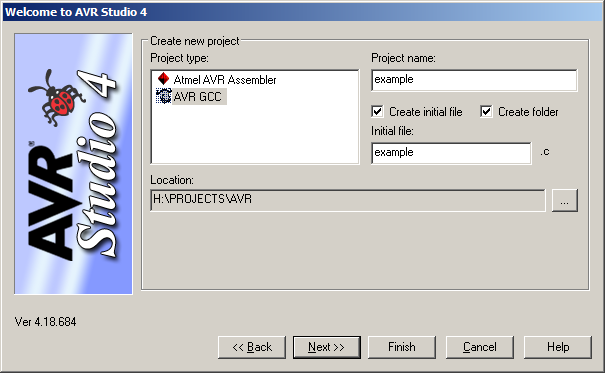
\includegraphics[scale=0.46]{newproject1}
  \caption{Eerste scherm bij aanmaken nieuw project}
  \label{fig:newproject1}
\end{figure}

\begin{figure}[h!]
  \centering
  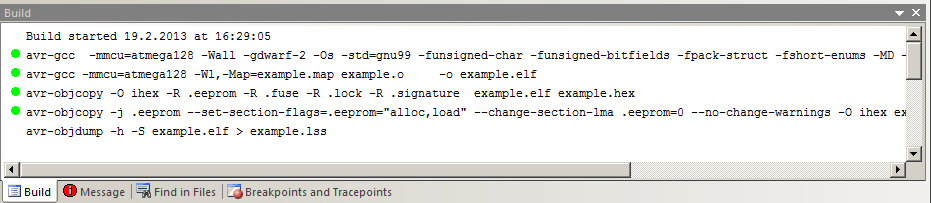
\includegraphics[scale=0.46]{atmega128gcc}
  \caption{De compiler genereert code voor de ATmega128}
  \label{fig:atmega128gcc}
\end{figure}

\section{Bij gebruik van interrupts lijkt het alsof de ATmega32 steeds herstart.}
Het gebruik van interrupts levert vele voordelen op. Maar het kan ook een bron zijn van
allerlei problemen. E\'{e}n van die problemen betreft de zogenaamde \textit{bad interrupt}.
Soms heb je het idee dat het programma op de AVR (met interrupts) opnieuw start. Bij debuggen
kom je er achter dat inderdaad de bekende gele pijl op de eerste instructie staat. Wat nu?
Dit kan gebeuren als je een interrupt aanzet (door middel van interrupt enble flags) waar
geen Interrupt Services Routine (ISR) voor is gedefinieerd. Er kan dus ook niet naar de ISR
gesprongen worden. De compiler lost die nogal rigoureus op door naar de reset vector te
springen. Een discussie over dit ''probleem'' is te vinden op
\url{http://savannah.nongnu.org/task/?7546}.

In het volgende voorbeeld is alleen de ISR voor de T/C1 Compare Match Interrupt gedefinieerd,
de ISR van de ADC Completion Interrupt is uitgecommentarieerd.

\begin{lstlisting}[style=numbers,caption=ISR vergeten]
#include <avr/io.h>
#include <stdint.h>
#include <avr/interrupt.h>

#define PRESCALER 1024UL
#define FREQ 10UL
#define LOAD ((F_CPU/(PRESCALER*FREQ))-1)

volatile uint8_t flag;
volatile uint16_t ADCval;

/* Compare A Match ISR */
ISR(TIMER1_COMPA_vect) {

	/* some code */
}

/* ADC ISR, signals new value is ready, copy value */
/*ISR(ADC_vect) {
	flag = 1;
	ADCval = ADC;
} */


int main() {

	/* Set up T/C1 */
	TCCR1A = (0<<WGM11)|(0<<WGM10);
	TCCR1B = (0<<WGM13)|(1<<WGM12)|(1<<CS12)|(0<<CS11)|(1<<CS10);
	OCR1A  = LOAD;
	TIMSK  = 1<<OCIE1A;

	/* Set up  ADC in single shot mode, select channel 0, interrupt */
	/* Refs is AREF, internal V off, ADC prescaler is 64 */
	ADMUX  = (0<<REFS1)|(0<<REFS0)|(0<<MUX4)|(0<<MUX3)|(0<<MUX2)|(0<<MUX1)|(0<<MUX0);
	SFIOR  = (0<<ADTS2)|(0<<ADTS1)|(0<<ADTS0);
	ADCSRA = (1<<ADEN)|(1<<ADSC)|(0<<ADATE)|(0<<ADIF)|(1<<ADIE)|(1<<ADPS2)|(1<<ADPS1)|(0<<ADPS0);

	/* Free interrupts */
	sei();

	/* Forever... */
	while (1) {
		/* code here */
	}

	return 0;
}
\end{lstlisting}

De compiler genereert een vector table waarin alle niet gedefinieerde vectoren
naar de \textit{default interrupt handler} verwijzen.

In onderstaande listing is een deel van de gegenereerde assemblercode afgebeeld
(deze file is te vinden met de extensie \texttt{.lss}, althans bij gebruik van
AVR Studio).

\begin{lstlisting}[language=AVR,caption=Deel van de assemblercode]
Disassembly of section .text:

00000000 <__vectors>:
   0:	0c 94 2a 00 	jmp	0x54	; 0x54 <__ctors_end>
   4:	0c 94 3c 00 	jmp	0x78	; 0x78 <__bad_interrupt>
   8:	0c 94 3c 00 	jmp	0x78	; 0x78 <__bad_interrupt>
   c:	0c 94 3c 00 	jmp	0x78	; 0x78 <__bad_interrupt>
  10:	0c 94 3c 00 	jmp	0x78	; 0x78 <__bad_interrupt>
  14:	0c 94 3c 00 	jmp	0x78	; 0x78 <__bad_interrupt>
  18:	0c 94 3c 00 	jmp	0x78	; 0x78 <__bad_interrupt>
  1c:	0c 94 3e 00 	jmp	0x7c	; 0x7c <__vector_7>       (*@ \label{asm1:isrtc1} @*)
  20:	0c 94 3c 00 	jmp	0x78	; 0x78 <__bad_interrupt>
  24:	0c 94 3c 00 	jmp	0x78	; 0x78 <__bad_interrupt>
  28:	0c 94 3c 00 	jmp	0x78	; 0x78 <__bad_interrupt>
  2c:	0c 94 3c 00 	jmp	0x78	; 0x78 <__bad_interrupt>
  30:	0c 94 3c 00 	jmp	0x78	; 0x78 <__bad_interrupt>
  34:	0c 94 3c 00 	jmp	0x78	; 0x78 <__bad_interrupt>
  38:	0c 94 3c 00 	jmp	0x78	; 0x78 <__bad_interrupt>
  3c:	0c 94 3c 00 	jmp	0x78	; 0x78 <__bad_interrupt>
  40:	0c 94 3c 00 	jmp	0x78	; 0x78 <__bad_interrupt>  (*@ \label{asm1:isradc} @*)
  44:	0c 94 3c 00 	jmp	0x78	; 0x78 <__bad_interrupt>
  48:	0c 94 3c 00 	jmp	0x78	; 0x78 <__bad_interrupt>
  4c:	0c 94 3c 00 	jmp	0x78	; 0x78 <__bad_interrupt>
  50:	0c 94 3c 00 	jmp	0x78	; 0x78 <__bad_interrupt>

00000054 <__ctors_end>:

; code skipped.

00000078 <__bad_interrupt>:
  78:	0c 94 00 00 	jmp	0	; 0x0 <__vectors>             (*@ \label{asm1:isrdef} @*)  
\end{lstlisting}

In de bovenstaande code is zien dat op regel \ref{asm1:isrtc1} een sprong
wordt gemaakt naar de ISR voor T/C1, maar in regel \ref{asm1:isradc} wordt
gesprongen naar de default interrupt handler. Deze routine staat beschreven
op regel \ref{asm1:isrdef} en zoals te zien is, wordt gesprongen naar adres
0. Daar wordt weer gesprongen naar de startup code.

\section{Debuggen gooit communicatie met de buitenwereld in de war.}
Als voorbeeld RS-232.

\section{Compiler-optimalisatie gooit debuggen in de war.}
Meestal werkt de code van een programma niet in \'{e}\'{e}n keer. Gelukkig is
er de mogelijkheid om de code te debuggen door stap voor stap door de coderegels
te lopen. Helaas zorgt compiler-optimalisatie voor problemen. Net als
bij \ref{sec:compopt} zet de compiler C-code om naar eigen inzicht. Dat
kan bijvoorbeeld zijn dat een \texttt{while}-lus wordt omgewerkt tot een
\texttt{do-while}-lus. Vaak is het dan niet mogelijk om \'{e}\'{e}n-op-\'{e}\'{e}n
de C-code te koppelen aan de gegenereerde assemblercode. Tijdens het debuggen
verdwijnt de gele pijl ineens. Soms komt deze dan weer terug, maar meestal moet
je het debuggen even pauzeren (en dan nog komt de pijl niet terug). De oplossing
is simpel: zet de compiler-optimalisatie uit. Dit kan je doen door optie
\texttt{-O0} in te stellen in de project-omgeving (in AVR Studio).

\bibliographystyle{plain}
\bibliography{CoderenopAVR}
 
\printindex

\end{document}
